% Created 2020-04-17 Fri 15:48
% Intended LaTeX compiler: pdflatex
\documentclass[presentation]{beamer}
\usepackage[utf8]{inputenc}
\usepackage[T1]{fontenc}
\usepackage{graphicx}
\usepackage{grffile}
\usepackage{longtable}
\usepackage{wrapfig}
\usepackage{rotating}
\usepackage[normalem]{ulem}
\usepackage{amsmath}
\usepackage{textcomp}
\usepackage{amssymb}
\usepackage{capt-of}
\usepackage{hyperref}
\usetheme{UoB}
\author{Mark Blyth}
\date{\textit{[2020-04-20 Mon]}}
\title{GPR Kernels}
\hypersetup{
 pdfauthor={Mark Blyth},
 pdftitle={GPR Kernels},
 pdfkeywords={},
 pdfsubject={},
 pdfcreator={Emacs 26.3 (Org mode 9.1.9)}, 
 pdflang={English}}
\begin{document}

\maketitle

\section{Background}
\label{sec:orgf6c7bd8}
\begin{frame}[label={sec:orgcc330c9}]{This week's goals}
\begin{itemize}
\item Rederive GPR for vector outputs
\begin{itemize}
\item Turns out this is an open problem
\item Hard to do generally, but I've found a way to avoid needing this
\end{itemize}
\item Get GPR to work
\begin{itemize}
\item Some success
\end{itemize}
\item Use it for a predictor-corrector
\begin{itemize}
\item Not got this far yet
\end{itemize}
\end{itemize}
\end{frame}

\section{Kernels}
\label{sec:orge3b22d2}
\begin{frame}[label={sec:org5a6045a}]{Model fitting -- it sort of works!}
\begin{center}
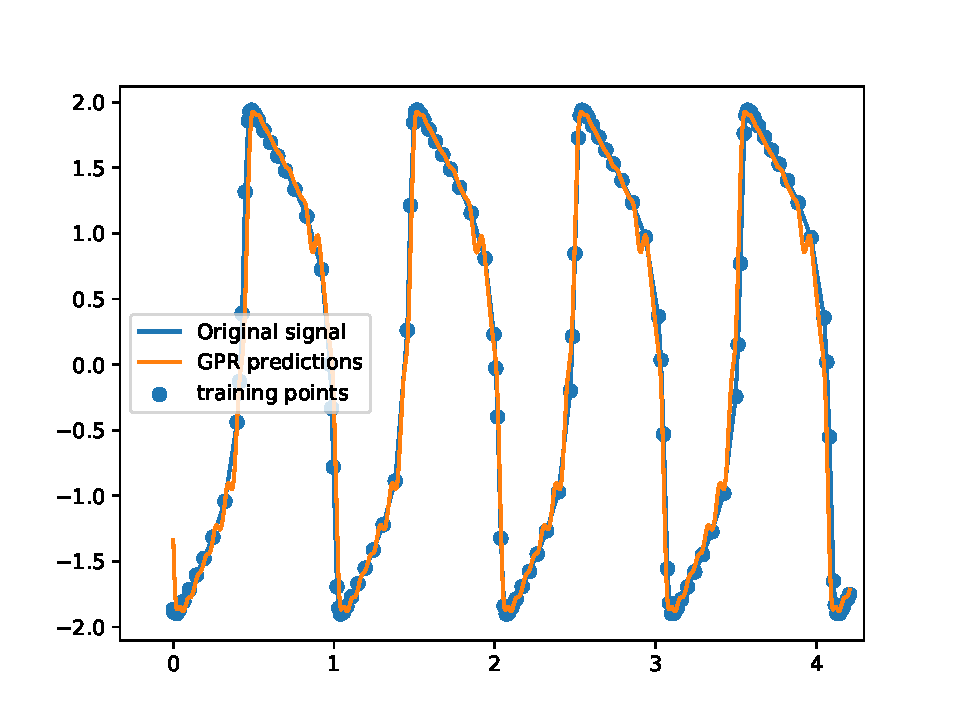
\includegraphics[height=.9\textheight]{./gpr1.pdf}
\end{center}
\end{frame}

\begin{frame}[label={sec:org773a803}]{30 seconds intro to Gaussian processes}
\begin{itemize}
\item Gives us a Gaussian distribution at any given time
\item That Gaussian distribution is the PDF of our function value at that time
\item Works by maintaining a probability distribution over candidate functions
\item Constructed by using Bayes' rule to condition on the evidence and form a posterior function distribution
\item Bayes' rule needs good priors!
\end{itemize}
\end{frame}

\begin{frame}[label={sec:org6d04eae}]{GPR kernels}
\begin{itemize}
\item They specify our prior distributions over functions
\item Good kernels = good priors = good results
\item (Kernels are interesting -- they implicitly encode an infinite dimensional feature space)
\end{itemize}
\end{frame}

\begin{frame}[label={sec:orgefb0037}]{Periodic kernels}
Data are periodic, so it makes sense to have a kernel that's periodic 

\begin{itemize}
\item If we choose a periodic kernel then we're favouring periodic functions in our prior function distribution
\item Periodic kernels give better fits on periodic data!
\item But, if the period isn't specified correctly, they'll give big errors and be harder to optimise\ldots{}
\end{itemize}
\end{frame}

\begin{frame}[label={sec:org2500959}]{Aperiodic kernels}
To avoid period-errors, use an aperiodic kernel and overlay each period's data on top of each other

\begin{itemize}
\item Aperiodic kernels don't encode our prior beliefs about periodicity, so they're not going to give as good a fit to the data
\item But, they have no period component, so they aren't sensitive to errors in the period
\item This means that in practice they can actually still give reasonable fits to the data
\end{itemize}
\end{frame}

\begin{frame}[label={sec:org85c95b7}]{Hyperparameters}
Both periodic and aperiodic kernels rely on hyperparameters; often\ldots{}
\begin{itemize}
\item \(l\): how similar nearby datapoints are
\item \(\sigma_f^2\): function amplitude
\item \(\sigma_n^2\): noise in the function observations
\end{itemize}

There's an interplay between kernel choice and hyperparameter selection:
\begin{itemize}
\item well-chosen kernels are easier to fit hyperparameters to; will still give good results with bad hyperparameters
\item bad kernels give bad results unless the hyperparameters are perfect, which is hard!
\end{itemize}
\end{frame}

\begin{frame}[label={sec:org28d3acd}]{Characteristic lengths}
\begin{columns}
\begin{column}{0.4\columnwidth}
\begin{center}
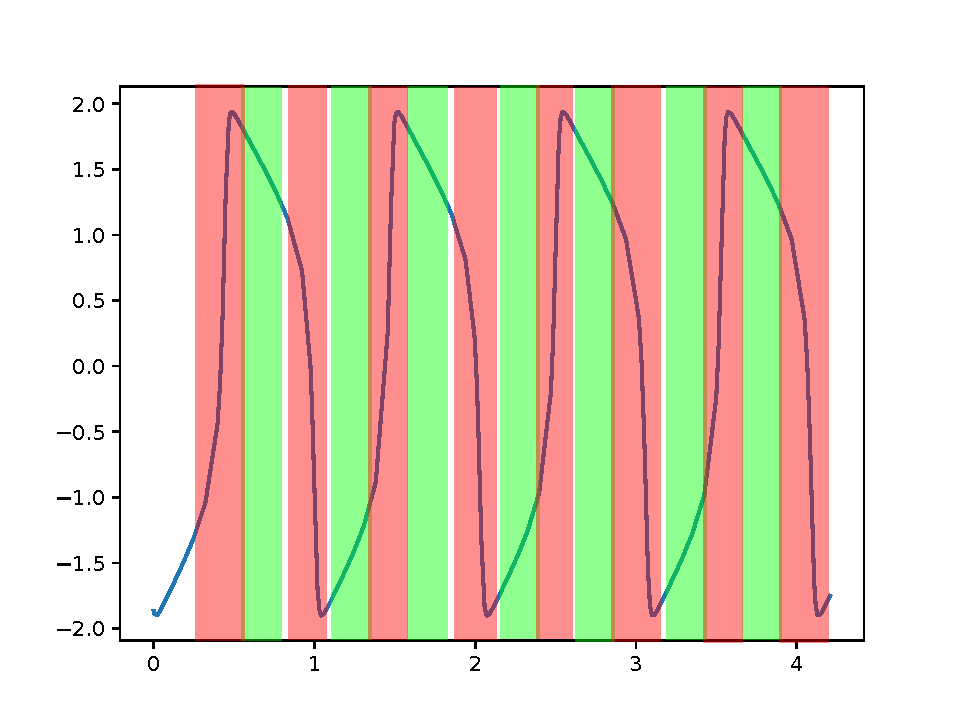
\includegraphics[width=\textwidth]{./ls.pdf}
\end{center}

\begin{center}
Bigger version on the next slide
\end{center}
\end{column}

\begin{column}{0.6\columnwidth}
\begin{itemize}
\item \(l\) is the most interesting hyperparameter
\item Measures how similar near-by datapoints are to each other
\item Since neurons are a multiple-timescale system, this isn't trivial
\item RED: points sampled close in time map to very different values, and are therefore dissimilar; small \(l\)
\item GREEN: points sampled close in time map to similar values; big \(l\)
\end{itemize}
\end{column}
\end{columns}
\end{frame}

\begin{frame}[plain,label={sec:org3de7fed}]{Characteristic lengths}
\begin{center}
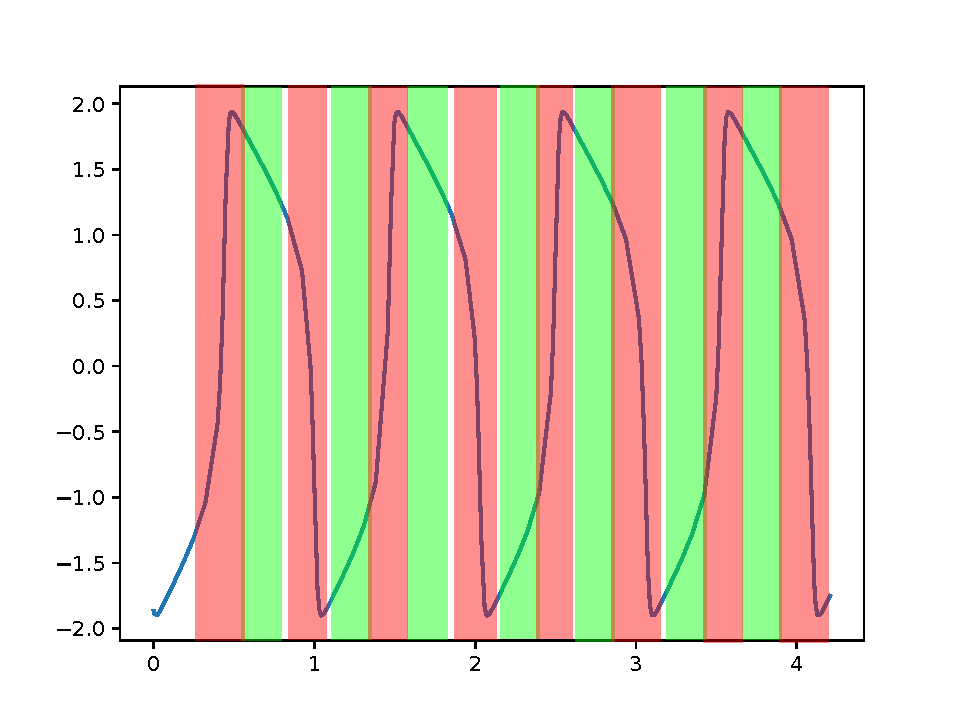
\includegraphics[height=1.2\textheight]{./ls.pdf}
\end{center}
\end{frame}

\begin{frame}[label={sec:org27c7500}]{The effects of \(l\)}
\begin{columns}
\begin{column}{0.7\columnwidth}
\begin{center}
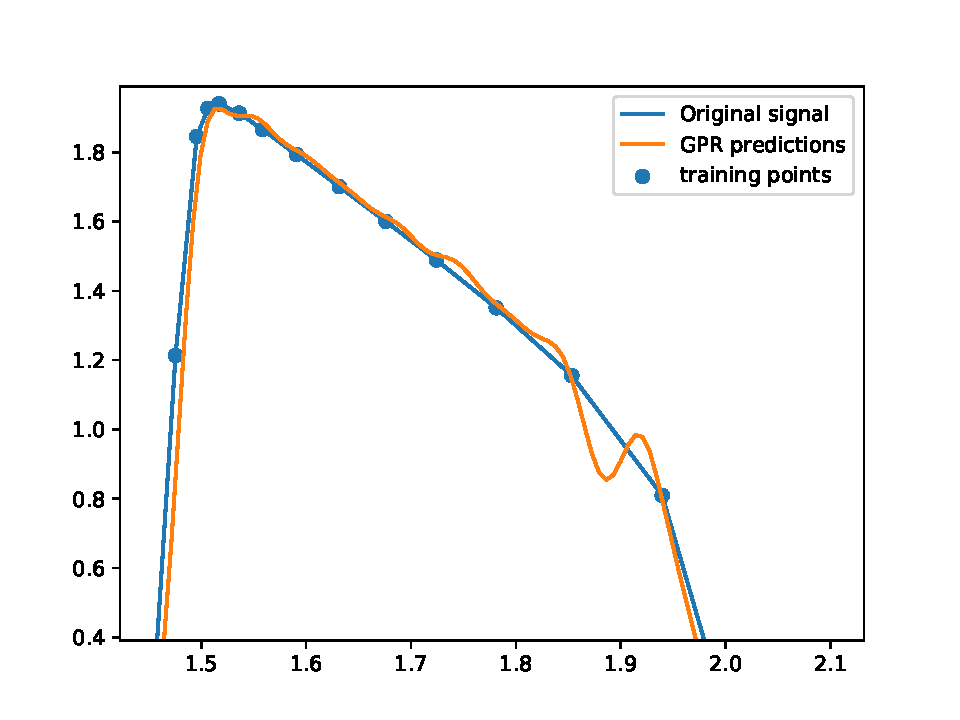
\includegraphics[width=.9\linewidth]{./gpr2.pdf}
\end{center}
\end{column}
\begin{column}{0.3\columnwidth}
\begin{itemize}
\item \(l\) varies across the signal
\item modelling with constant \(l\) gives bad results
\end{itemize}
\end{column}
\end{columns}
\end{frame}

\begin{frame}[label={sec:org9112c1b}]{Solution}
There's kernels for modelling variable \(l\), but\ldots{}
\begin{itemize}
\item \(l\) becomes a function in space
\item No longer a single hyperparameter to fit, but an enitre hyperfunction
\item Hyperparameter space goes from 3-dimensional to infinite!
\item One approach models the \(l\) function as a Gaussian process, and demonstrates an efficient / computationally tractable way of fitting it
\item The paper is hard
\end{itemize}
\end{frame}

\begin{frame}[label={sec:orga094890}]{Generalised spectral mixture kernels}
\begin{itemize}
\item Use GPR to generate a kernel for the specific input data
\item Provides a tractable way of fitting this kernel
\item Once fitted for one periodic orbit, it will still work well for the rest
\item Automatically deals with periodicity, non-stationarity, so we resolve the periodic kernel dilemma!
\end{itemize}

Remes, Sami, Markus Heinonen, and Samuel Kaski. "Non-stationary spectral kernels." Advances in Neural Information Processing Systems. 2017.
\end{frame}


\section{Next steps}
\label{sec:org179cbc4}
\begin{frame}[label={sec:orgebbee8a}]{Next steps}
\begin{itemize}
\item Work through the paper to understanding
\begin{itemize}
\item Might take a while!
\end{itemize}
\item Implement a GSMKernel
\begin{itemize}
\item This should finish off the the GPR part
\item If GPR turns out to be a no-go, the rest of the predictor/corrector scheme will still work with another interpolating model, eg. periodic splines
\end{itemize}
\item Code up a predictor
\begin{itemize}
\item Should be trivial once GPR is sorted
\end{itemize}
\item Code up a corrector
\begin{itemize}
\item Should be interesting but very doable
\end{itemize}
\end{itemize}
\end{frame}
\end{document}
